\documentclass[12pt,fleqn]{article}\usepackage{../../common}
\begin{document}
Materyel Mekaniği - 1

Alan Atalet Momenti (Area Moment of Inertia)

Herhangi bir şekil için, o şekilde olan bir eksene olan uzaklık karesinin alan
üzerinden entegre edilmesiyle ``alan atalet momenti'' sonucu elde ediliyor
[3, sf. 362]. 

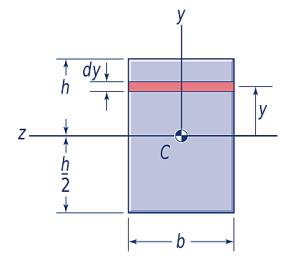
\includegraphics[width=10em]{phy_020_strs_00_04.jpg}

Formül, $z$ eksen bazlı olarak

$$
I_z = \int_A y^2 \ud A
$$

Bu entegral belli şekiller / alanlar için muhakkak hep aynı olur. Üstteki kalıp
bazı alanlarda, mesela inşaat mühendisliğinde, çok ortaya çıktığı için
bilinir, ve belli şekiller için $I$ formülü önceden hesaplanmıştır.

Üstteki basit bir şekil tabii ki, ama onun da bir formülü var, eğer türetmek
istersek,

$$
I_z = \int_{-h/2}^{h/2} y^2 (b \ud y) = b \frac{y^3}{3} \bigg\vert_{-h/2}^{h/2} =
\frac{b h^3}{12}
$$

Yani dikdörtgensel şekiller için $I_z$ gerektiğinde hemen üstteki formül
kullanılabilir. Dairesel, üçgensel, vb. pek çok şekil için bu hesap mevcut.

Eksenel Yükleme (Uniaxial Loading)

Pek çok problemde kullanılan en temel deformasyon (yamulma, şekil değiştirme)
türü altta görülen tür yüklemedir. Bir demir, ya da plastik çubuk iki kuvvetle
boyu yönünde (tek bir eksende yani) iki tarafa doğru çekilir, bizim
ilgilendiğimiz çubukta seçilen herhangi bir noktanın nereye gittiği, yani o tek
eksendeki deformasyonun ne olduğu.

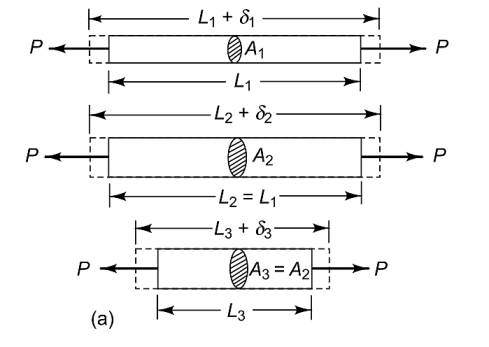
\includegraphics[width=20em]{phy_020_strs_00_01.jpg}

Diyelim ki üstteki her üç çubuk aynı maddeden yapılmış, farklı uzunlukları ve
kalınlıkları var, her çubuğa sıfırdan başlayarak belli seviyelerde $P$ kuvveti
ile yük uyguluyoruz, ve çubuğun uzunluk değişimi (elongation) $\delta$
değerinin, ki tek boyuttaki deformasyon budur, ne olduğuna bakıyoruz. Her 1,2,3
çubuğu için $P/A$ ve $\delta/L$ değerlerini grafiklersek çoğunlukla sonuç ya alt
soldaki gibi ya da sağdaki gibi çıkacaktır [1, sf. 76].

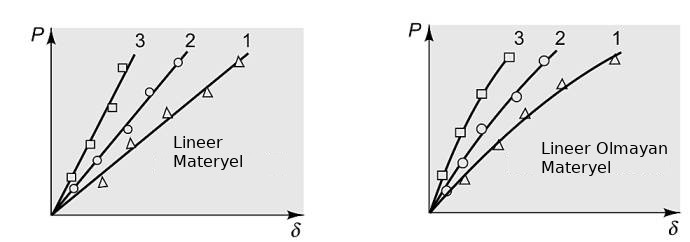
\includegraphics[width=20em]{phy_020_strs_00_02.jpg}

Eğer materyelin eksenel yük ve uzama ilişkisi lineer ise o zaman sonuç soldaki
resim gibi çıkar. Grafiğin eğimine elastiklik genliği (modulus of elasticity)
adı verilir ve çoğunlukla ona $E$ sembolü verilir. Formülsel olarak belirtirsek,

$$
E = \frac{P/A}{\delta / L}
\mlabel{1}
$$

$E$ formülüne Young'in Genliği (Young's Modulus) ismi de verilir. 

$\delta/L$ büyüklüğü mevcut büyüklüğe nazaran ne kadar uzama olduğunu gösteren
bir oran, mesela 200 cm için 2 cm büyüme var ise 2/200, bu bir tür yüzde hesabı
olarak görülebilir (ek olarak yüz ile de çarpmak gerekir ama aşağı yukarı öyle).

Not: $P$ çoğunlukla basınç (pressure) için kullanılır ama burada kuvvet.

$P/A$'nin birimi kuvvet bölü birim alan olduğu ve $\delta / L$ birimsiz olduğu
için $E$'nin birimi de kuvvet bölü birim alan olacaktır. Daha ileride göreceğiz
ki $P/A$ bir alan $A$ üzerindeki ortalama {\em stres} değeridir, $\delta / L$
ise $L$ boyunca hissedilen {\em gerinim} değeridir (strain).

Yani $E$ birimi Newton bölü metrekare olacaktır, $N/m^2$ ya da Pascal, Pa terimi
kullanılabilir. Bazı tipik değerler demir ve çelik için $200\cdot 10^6$ kilo
Newton / $m^2$, aliminyum için $69 \cdot 10^6$ $kN / m^2$.

(1) formülünü düzenleyip tekrar yazarsak, 

$$
\delta = \frac{PL}{AE}
$$

Üstteki formül Hooke Kanunu'nun basit bir formudur aslında; bu isim Robert Hooke
bilimcisine atfendir, ki pek çok materyelin yük-deformasyon eğrisinin lineer
olduğunu keşfeden Hooke'tur. Bu arada materyelin eğrisi lineer ise bu durum
sarma yaylar (coiled springs) için de aynıdır. Kavramsal ve formülsel olarak
bir demir çubuğu yay olarak görsek mesela $10^3 mm^2$ genişliğinde ve
1 metre uzunluğunda, Hooke Kanunu

$$
F = k x
$$

ki $F$ kuvvet, $k$ yay sabiti ve $x$ uzama, mevcut semboller ile,

$$
P = k \delta
$$

$$
k = \frac{P}{\delta}
$$

$$
= \frac{P}{PL / AE} = \frac{1}{L / AE} = \frac{AE}{L} =
\frac{10^3 10^{-3} 205}{1} =
205 GN/m
$$

Çubuk Bükülme Gerinimi (Beam Bending Strain)

Daha önce gördüğümüz üzere bir normal gerinim $\epsilon$'nin baz tanımı

$$
\epsilon = \Delta L / L
\mlabel{2}
$$

ki $L$ mevcut uzunluk, $\Delta L$ uygulanan kuvvet sonucu elde edilen uzama [2].
Bu formülü ufak bir demir çubuk parçasının bükülmesine uygulayabilir miyiz
acaba? 

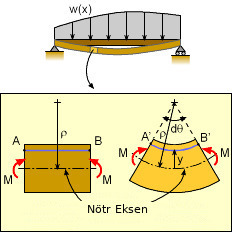
\includegraphics[width=15em]{phy_020_strs_00_03.jpg}

Üstteki resme göre formülleri yazabiliriz. Gösterilen çubuk herhangi bir
çubuk, tipi ve onun üzerindeki yükün dağılımı farketmiyor.

Resimde alt solda bükülme öncesi, sağda sonrası görülüyor, bükülme nötr eksenden
$\rho$ uzaklığındaki bir nokta etrafında ve $\ud\theta$ kadar. $\rho$'ya bükülme
çemberinin / eğiminin yarıçapı (radius of curvature) ismi de verilir. Bükülme
öncesi $AB$ uzunluğu mesela görülen mavi çizgi için $A'B'$ haline gelecek. Ama
dikkat edersek nötr eksene yakın noktalar daha az uzayacak, uzaklar daha
fazla.. bu uzaklığı bir $y$ üzerinden temsil edebiliriz. O uzaklığı hesaba katan
bir gerinim formülü nasıl elde ederiz?

Nötr eksene $y$ uzaklığındaki $AB$ bükülme sonrası $A'B'$ oldu ise, bu durumu
(2) bazında belirtelim,

$$
\epsilon = \frac{A'B' - AB}{AB}
$$

Şimdi $A'B'$ hesabına gelelim. Dikkat edersek $A'B'$ ufak bir çember çevresi,
verili yarıçapı ve açı üzerinden bu çember çevresi hesaplanabilir, tüm daire
çevresi muhakkak $2 \pi r$, açısı bilinen ufak parçalar için $\pi \theta$,
burada açı $\theta$ tüm $2 \pi$'ye oranlı, radyan olarak. O zaman

$$
AB = \rho \ud \theta
$$

$A'B'$ için ufak dairenin yarıçapı değişir, nötr eksene $y$ kadar uzak isek,
$A'B'$ yarıçapı $\rho - y$, demek ki 

$$
A'B' = (\rho - y) \ud \theta
$$

Bunları (2)'ye koyarsak,

$$
\epsilon = \frac{(\rho - y) \ud \theta - \rho \ud \theta}{\rho \ud\theta} =
\frac{\rho \ud\theta - y \ud\theta - \rho \ud\theta}{\rho \ud\theta} =
- \frac{y \ud\theta}{\rho \ud\theta}
$$

$$
\epsilon = - \frac{y}{\rho}
$$

Üstteki gerinim formülünü stres formülüne dönüştürebiliriz, Hooke'un Kanunu
$\sigma = E \epsilon$ üzerinden,

$$
\sigma = -E y / \rho
\mlabel{3}
$$

Fakat bu formülün bazı dezavantajları var, mesela bükülme eğimin yarıçapı
$\rho$'yu bulmak zor. Acaba bükülme momenti (bending moment) ile bir ilişki
kurarak eğim yarıçapından kurtulabilir miyiz?

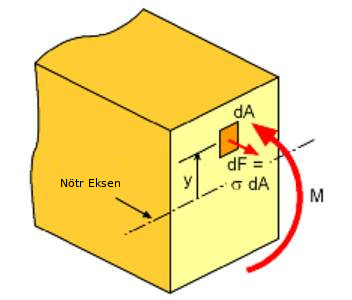
\includegraphics[width=10em]{phy_020_strs_00_05.jpg}

Nötr eksen etrafındaki bükülme momenti

$$
M = \int y (-\ud F)
$$


$\ud F$ bükülme sebebiyle sonsuz küçük alan $\ud A$ üzerinde etkili olan
kuvvettir. Tabii stres kuvvet bölü alandır o zaman ters yönde de gidebiliriz,
stres çarpı alan kuvvettir, yerine koyalım,

$$
M = -\int y \sigma \ud A
$$

$\sigma$ için (3) formülünü koyalım,

$$
\frac{E}{\rho} \int y^2 \ud A = M
$$

Formülde bir alan atalet moment kalıbı gözüküyor, ona $I$ diyelim,

$$
M = E I / \rho
$$

Üstteki formül [3, sf. 464] kaynağında moment-eğri (moment-curvature) denklemi
olarak tarif ediliyor, şu şekilde de bulunabilir [6, sf. 363] ,

$$
\kappa = \frac{1}{\rho} = \frac{M}{EI}
$$

Ama $\rho$'dan hala kurtulamadık, (3)'u $\rho$ için düzenleyip üstteki formüle
sokarsak,

$$
EI / (-Ey / \sigma )  = M
$$

Basitleştirince

$$
\sigma = - \frac{M y}{I}
$$

Bu formül bükülme normal stres (flexure) formülüdür [2], [6, sf. 364].

Gerinim Enerji Yoğunluğu (Strain Energy Density)

Yapılan iş ve enerji arasındaki bağlantıyı işledik. Şimdi bir maddeye uygulanan
stres ve onun sebep olduğu gerinimin yol açtığı esnemeden bahsedelim, bir kuvvet
uygulanıyor ve bir esneme oluyor, bu hesap kuvvet çarpı mesafe ile yapılan iş
olarak hesaplanabilir. Diyelim ki bir çubuk (bar) üzerinde tek eksenel $P$
kuvveti uygulanıyor, sonucunda $\ud \Delta$ kadar uzama var [4, sf. 243],

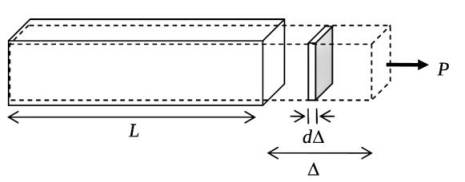
\includegraphics[width=20em]{phy_020_strs_00_07.jpg}

Yapılan iş

$$
\ud W = P \ud \Delta
$$

Eğer $P$ sürekli uygulansa ve uzama devam etse tüm ufak uzamalar üzerinden
yapılan iş $\ud \Delta$ üzerinden bir entegral gerektirir, fakat alttaki
gibi basit durumda sadece üçgen alan hesabı yeterli,

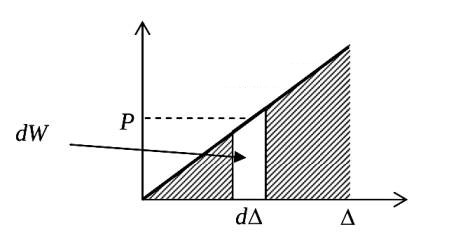
\includegraphics[width=20em]{phy_020_strs_00_08.jpg}

Şu formülü kullanabiliriz,

$$
U = \frac{1}{2} P \Delta
$$

Önceden hatırlarsak $\Delta = PL / EA$ idi, o zaman üstteki 

$$
U = \frac{P^2 L}{2 E A}
\mlabel{4}
$$

olur.

Yoğunluğa gelirsek; gerinim enerjisi madde içinde farklı seviyelerde olabilir,
onu sonsuz ufak bir hacim için hesaplarız ve gerektiğinde sonrada tüm enerji
için tüm hacim üzerinden entegre ederiz.

Alttaki çubuktaki ufak bir hacim birimine bakalım, birimin kenarları $\ud x$,
$\ud y$, $\ud z$ büyüklüğünde, birimin hacmi tabii ki $\ud V = \ud x \ud y \ud
z$.

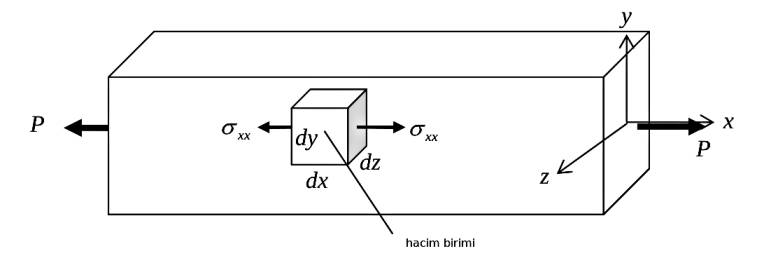
\includegraphics[width=25em]{phy_020_strs_00_06.jpg}

Formül (4) kullanalım, stres için $\sigma$ sembolü kullanacağız, stres kuvvet
bölü alan demektir, ufak birimdeki alan $A = \ud y \ud z$, o zaman
$P = \sigma_{xx} \ud y \ud z$, üstteki ufak birimdeki gerinim enerjisi

$$
U = \frac{(\sigma_{xx} \ud y \ud z)^2 \ud x}{2 E \ud y \ud z} =
\frac{\sigma_{xx}^2 \ud y^2 \ud z^2 \ud x}{2 E \ud y \ud z} =
\frac{\sigma_{xx}^2 \ud y \ud z \ud x}{2 E} 
$$

$$
= \frac{\sigma_{xx}^2 \ud V}{2 E} 
$$

Yoğunlukla ilgileniyoruz demiştik, bize birim hacimdeki $U$ lazım, o zaman
yoğunluk $u$

$$
u = \frac{\sigma_{xx}^2}{2 E}
$$

Hooke Kanunu $\sigma_{xx} = E \epsilon_{xx}$ üzerinden üstteki son formül,
gerinim enerji yoğunluğu

$$
u = \frac{1}{2} \sigma_{xx} \epsilon_{xx}
$$

olarak ta gösterilebilir. Alttaki resimde görülebileceği gibi bu tek eksenel
stres-gerinim eğrisinin altında kalan alandır,

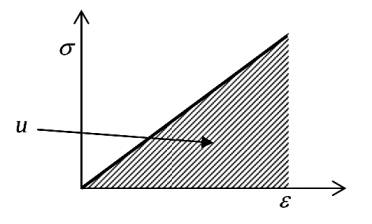
\includegraphics[width=15em]{phy_020_strs_00_09.jpg}

Daha çetrefil $\sigma-\epsilon$ ilişkileri (ve eğrileri) için $u$ hesabı
bir entegral olacaktır,

$$
u = \int_{0}^{\epsilon_{T}} \sigma_{xx} \ud \epsilon_{xx} 
$$

Gerinim, esneme, enerji alakası şöyle de görülebilir, uygulanan stresin
oluşturduğu esneme bir iş yapıyor, bu iş ile enerjiyi esnemeye transfer
ediyoruz, bir lastiği uzattığımızda enerji o lastiğin ``elastisitesine''
aktarılıyor sanki, bu işin / enerjinin birim hacimdeki ölçüsü gerilim
enerji yoğunluğunu veriyor bize.

İlerlemeden önce birazdan lazım olacak iki formülü bulalım. Daha önce gördük ki

$$
I = \int \int X_2^2 \ud X_2 \ud X_3
$$

ve

$$
M = \int \int -X_2 \sigma_{11} \ud X_2 \ud X_3
$$

Üstteki iki formülü birleştirelim, $M$ içinde $I$ oluşturalım, ve yerine koyalım,

$$
M = \int \int -\frac{X_2}{X_2^2} X_2^2 \sigma_{11} \ud X_2 \ud X_3 =
-\frac{1}{X_2} \sigma_{11} I 
$$

Buradan $\sigma_{11}$ eşitliğine geçilir,

$$
\implies \sigma_{11} = -\frac{M X_2}{I}
$$

Yatay Kesme Stresi

Kesme stresi $\tau$'yu bulmak için yine kirişin ufak bir kısmına odaklanalım,

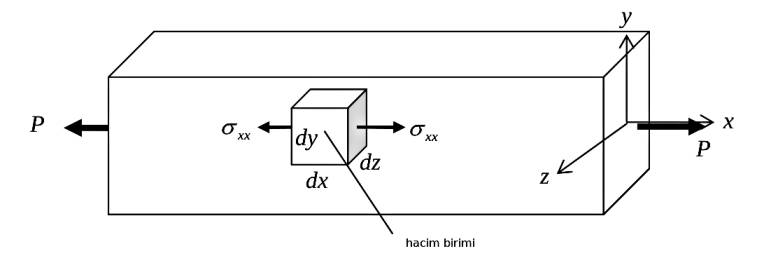
\includegraphics[width=15em]{phy_020_strs_00_06.jpg}

Tüm etki eden kuvvetlerin toplamı sıfır olmak zorundadır [2],

$$
-P + (P + \ud P) + \tau b \ud x = 0
$$

$$
-\ud P/\ud x = \tau b
\mlabel{1}
$$

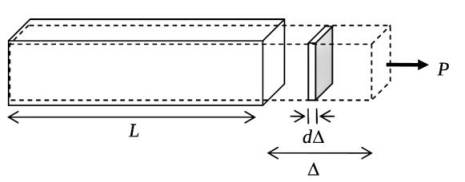
\includegraphics[width=15em]{phy_020_strs_00_07.jpg}

$P$'yi bulmak için $A$ bölgesindeki stresleri entegre ediyoruz,

$$
\int_A \ud P = \int_A \sigma_b \ud A
$$

Fakat daha önce bulduk ki $\sigma_b = -My / I$, yerine koyunca,

$$
P = \int_A - \frac{My}{I} \ud A
$$

$M$ ve $I$ sabittir, entegral dışına çıkartılabilir,

$$
P = - \frac{M}{I} \int_A y \ud A = - \frac{MQ}{I}
$$

Üstte bulunan $P$'yi (4)'e sokunca,

$$
- \frac{\ud}{\ud x} \left( - \frac{MQ}{I} \right) = \tau b
$$

$$
\frac{Q}{I} \frac{\ud M}{\ud x} = \tau b
$$

Şimdi hatırlarsak $\ud M/\ud x$ türevi yatay kesme / teğetsel yükü $V$'ye
eşittir. O zaman

$$
\frac{Q}{I} V = \tau b
$$

Nihai yatay kesme stres denklemi,

$$
\tau = \frac{V Q}{I b}
$$

Kaynaklar

[1] Crandall, {\em An Introduction to the Mechanics of Solids}

[2] Gramoll, {\em Mechanics},
    \url{http://www.ecourses.ou.edu/cgi-bin/ebook.cgi?topic=me}

[3] Craig, {\em Mechanics of Materials, Third Edition}

[4] Kelly, {\em University of Auckland, Solid Mechanics, Part I}

[6] Gere, {\em Mechanics of Materials}

[7] Khennane, {\em Introduction to Finite Element Analysis using Matlab and Abaqus}

\end{document}
